% !TeX root = main.tex

\section{Approach}
\frame{\frametitle{Outline} 
	\small
	\tableofcontents[
	currentsection,
	subsectionstyle=show/shaded/hide
]}

\subsection{Architecture}
\begin{frame}{\insertsubsection}
	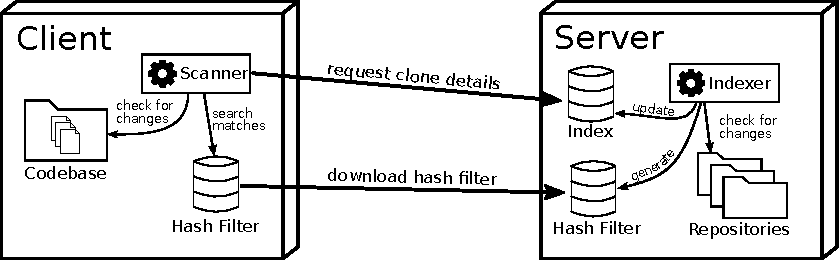
\includegraphics[width=\linewidth]{../written/figures/architecture_overview.pdf}
	\begin{description}
		\small
		\item[Target System] System on client which should be scanned for copied code
		\item[Reference System] Open source software system on server
	\end{description}
\end{frame}

\subsection{Index Creation}
\begin{frame}{\insertsubsection}
	For each file of each reference system:
	\begin{enumerate}
		\item Normalize source code files
		\item Group statements into chunks
		\item Hash normalized chunks of code
		\item Store location of chunk in index using hash as key for the key-value store
	\end{enumerate}
\end{frame}

\subsection{Normalization}
\begin{frame}{\insertsubsection}
	Focus on features and properties relevant for comparing copied code.\\
	\vspace{5mm}
	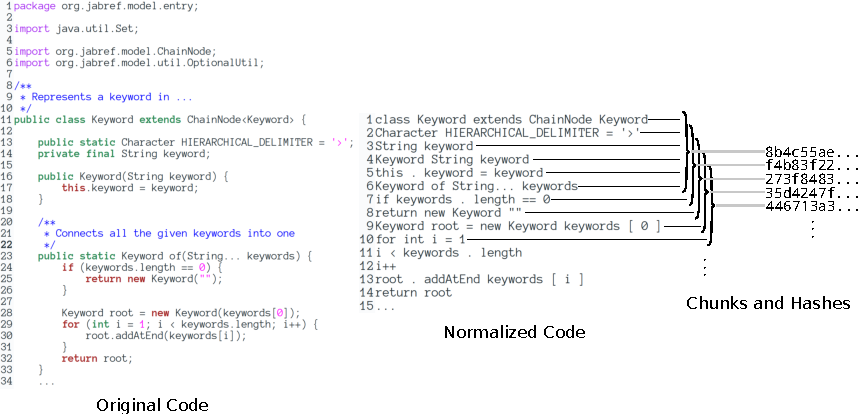
\includegraphics[width=\linewidth]{../written/figures/normalization.pdf}
\end{frame}

\subsection{History Analysis}
\begin{frame}{\insertsubsection}
	\begin{itemize}
		\item Analyzing history relevant to find old versions of a file
		\item Granularity of indexing can be fine or gross: Commit based or specific versions
		% TODO How is it done?
	\end{itemize}
\end{frame}

%TODO Problem with tags

\subsection{Hash Filter}
\begin{frame}{\insertsubsection}
	\textbf{Problem:} Lots of request have to be sent to server\\
	\pause
	\vspace{2mm}
	\textbf{Solution:} Bloom filter on client side
	\vspace{2mm}
	\begin{itemize}
		\item Data structure, which can be downloaded to client
		\item Client can decide whether a hash is part of the index with very small false positive probability
		\item Fraction in size compared to the index database
		\item Reduces number of requests to a fraction
	\end{itemize}
\end{frame}

\subsection{Searching for Copied Code}
\begin{frame}{\insertsubsection}
	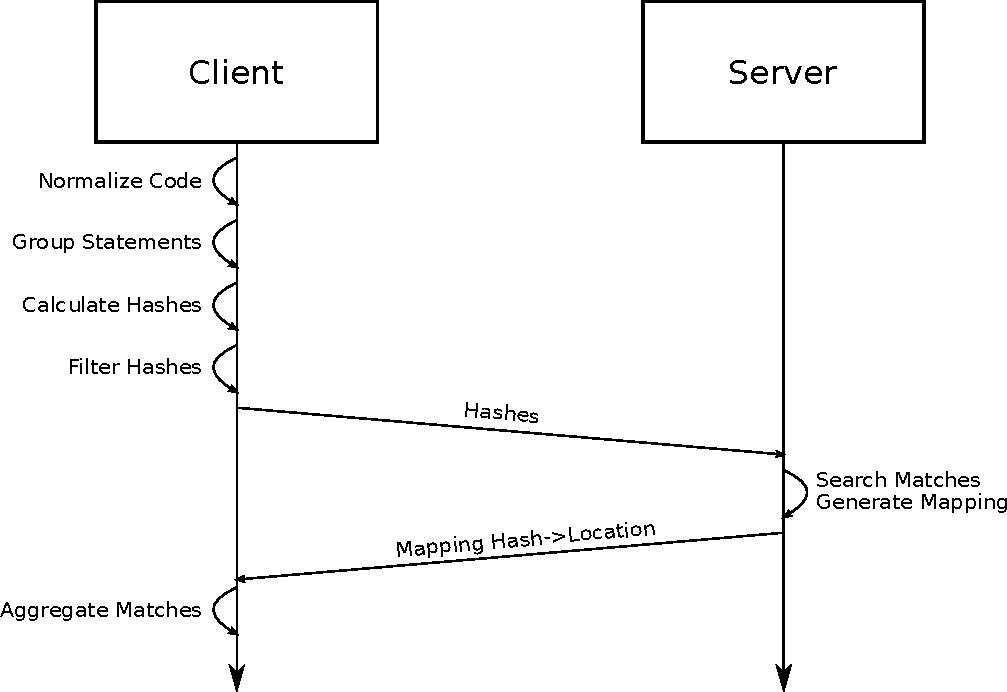
\includegraphics[width=\linewidth]{../written/figures/searching_copied_code.pdf}
\end{frame}

%TODO aggregation?
